\documentclass[12pt]{article}

\usepackage{upgreek}

\usepackage{amsmath}

\usepackage{graphicx}
\graphicspath{ {imgs/} }

\usepackage{dsfont}

\usepackage{mathtools}

\usepackage{hyperref}

\usepackage[utf8]{inputenc}

\usepackage{mathtools}

\usepackage{textcomp}

\usepackage[english]{babel}

\usepackage{tikz}

\usepackage{tcolorbox}

\usepackage{amsthm,amssymb}

\setlength{\parindent}{0cm}

\renewcommand\qedsymbol{$\blacksquare$}

\usepackage{fancyhdr}
 
\pagestyle{fancy}
\fancyhf{}
\fancyhead[LE,RO]{Graph Theory -- Fall 2017}
\fancyhead[RE,LO]{Joshua Concon}
\fancyfoot[CE,CO]{\leftmark}
\fancyfoot[LE,RO]{\thepage}


\begin{document}

\title{MATC32: Graph Theory\\ Lecture Notes}
\date{University of Toronto Scarborough -- Fall 2017}
\author{Joshua Concon}
\maketitle
Pre-reqs are MATB24, which is the second course on linear algebra at UTSC.
Instructor is Dr. Louis de Thanhoffer de Volcsey. I highly recommend sitting at the front since he likes to teach with the board. If you find any problems in these notes, feel free to contact me at conconjoshua@gmail.com.

\tableofcontents

\pagebreak

\section{Tuesday, September 5, 2017}

\subsection{The Seven Bridges of Konigsberg}

So basically there's this city called Konigsberg where a river flows through, and because of that, there are 7 bridges in the city. The bridges look like this:\\
\\
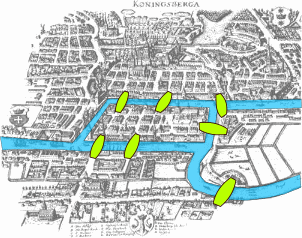
\includegraphics{Konigsberg_bridges}\\
\\

There problem that came up is whether or not it was possible to walk through every bridge in the city once in the same walk. This problem was eventually solved by Euler.\\
\\
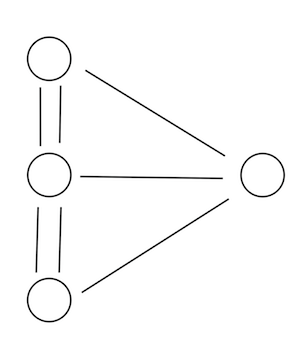
\includegraphics{Konigsberg_bridges_graph}\\
\\
It can be simplified to this. This is called a 'Graph', the circles are called 'nodes' or 'vertices' and the lines are called 'edges'. The different parts of the city are represented by the nodes and the bridges are represented by the edges.\\
\\
\begin{tcolorbox}[title=Definition: Graph ($G$)]
	\begin{enumerate}
		\item{Contains a set $V(G) =$ the set of nodes}
		\item{Contains a set $E(G) =$ the set of edges}
	\end{enumerate}
	A graph is called \textbf{Simple} if the graph has no loops and does not have multiple edges (i.e. Each edge is an unordered pair of distinct vertices).\\
	A graph is called a \textbf{Loop} if there is an edge that connects a vertex to itself.
\end{tcolorbox}

\begin{tcolorbox}[title=Definition: Path]
	A set of edges denoted by vertices $v_1, v_2, ..., v_n$ where there is a node between every edge between $v_i$ and $v_{i+1}$ $\forall i, 1 \leq i \leq n-1$
\end{tcolorbox}

\subsection{(Outline) Solution to Konigsberg}

Assume the graph has a path containing all edges $u_1,...,u_n$.\\
\\
Consider a vertex that isn't the first or last vertex travelled in the path (i.e. any vertex excluding $u_1$ and $u_n$).\\
\\
There must be an even number of edges for each of the nodes in between the edges in the path (excluding the first and the last node visited, unless the first and the last node visited are the same node).\\
\\
Since there are an odd number of adjacent nodes for all 4 nodes, this path does not exist. Therefore, there is no solution to Konigsberg.

\newpage

\section{Friday, September 8, 2017}

\subsection{Graphs}

\begin{tcolorbox}[title=Definition: Graphs]
	A graph $G$ consists of 2 (finite) sets:
	\begin{itemize}
		\item{$V(G)$ : vertex set}
		\item{$E(G)$ : edge set}
	\end{itemize}

	Together with an assignment from $E(G)$ to the set of subsets $V(G)$, where the subset is of size 1 or 2, containing the node(s) at the ends of the endpoints of each edge.
\end{tcolorbox}

If an edge has the same node at both of it's endpoints, it is called a \textbf{loop}.\\
\\
If 2 vertices are endpoints of more than one edge, we say that they are \textbf{multiply-edged}.\\
\\
A graph without multiply-edged vertices is called \textbf{simple}.\\
\\
\underline{Example:}


\includegraphics[scale=0.125]{lec2-1}

$$E(G) = \{ e_1, ... , e_7 \}$$
$$V(G) = \{ N_1, ... , N_4 \}$$

some of the assignments of $E(G) \mapsto V(G)$ include:
$$e_5 \mapsto \{ N_1, N_4 \}$$

\textbf{Adjacent edges} are edges with a vertex that is a common endpoint.

\subsection{Graph Theory Applications}

\subsubsection{Uber}

$$V = \text{People Using Uber (both drivers and passengers)}$$
$$E = \text{If it is realistic for a driver to pick up a person}$$

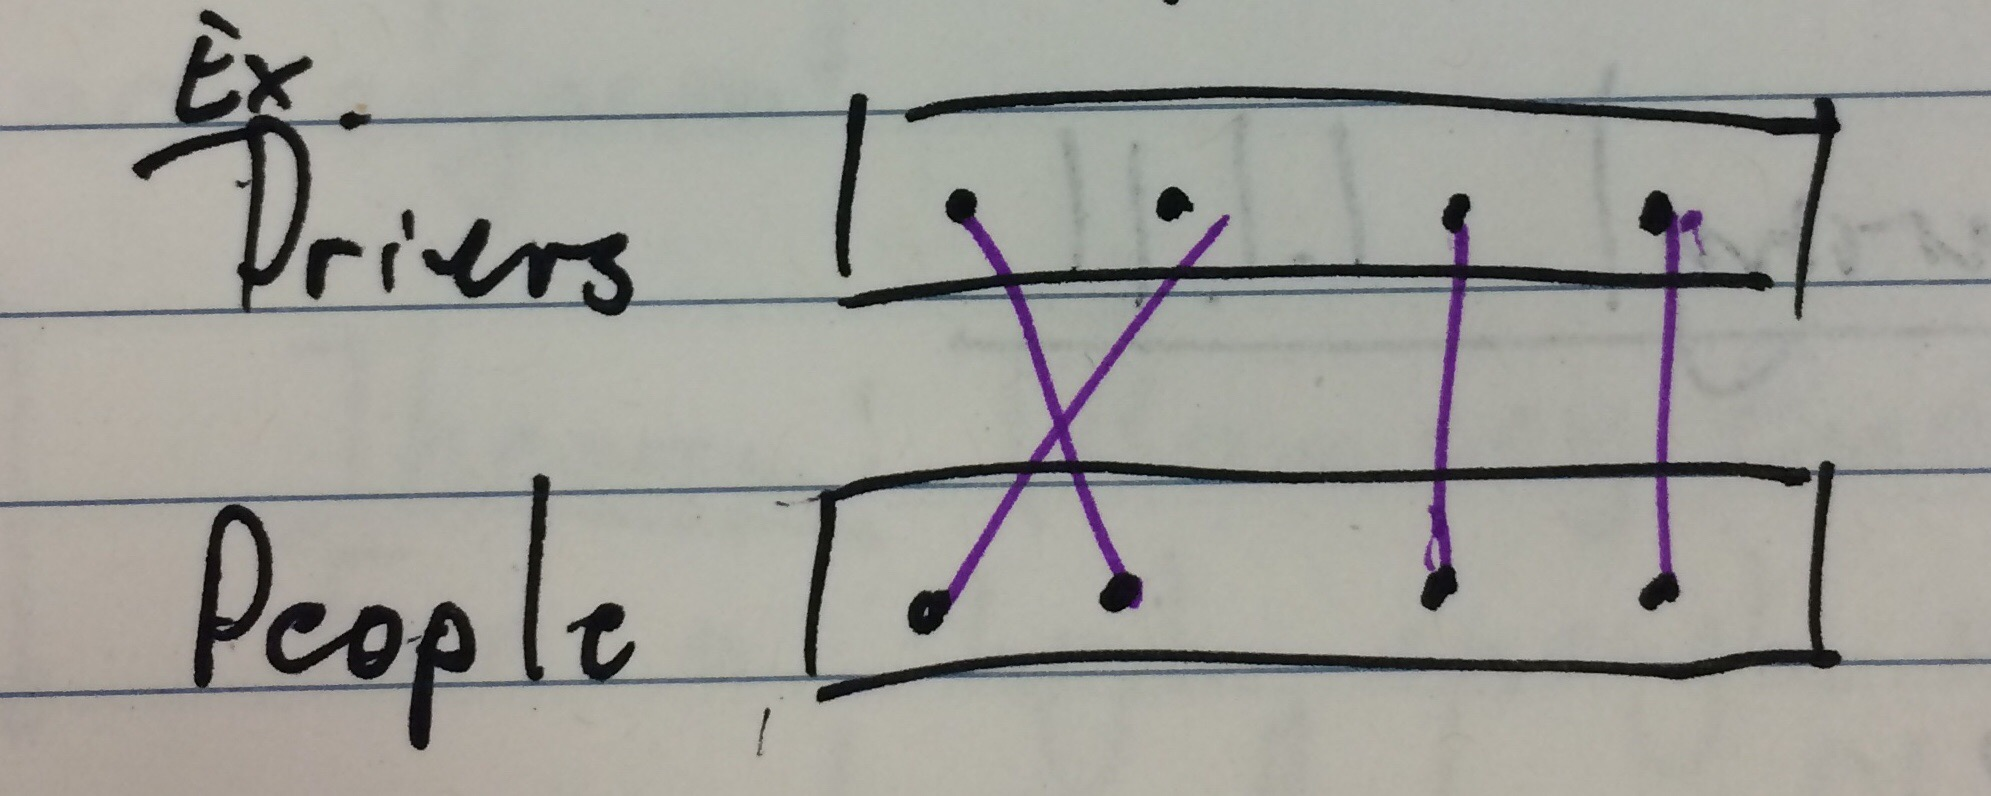
\includegraphics[scale=0.125]{lec2-2}

\begin{tcolorbox}[title=Definition: Matching]
	A \textbf{matching} in a group is a set of edges, none of which are adjacent
\end{tcolorbox}

\underline{Note:} $V(G) = S_1 \sqcup S_2$ and there are no edges between of $S_1$ with respect to $S_2$ ($\sqcup$ : refers to a union between two disjoint sets).\\
\\
These two sets $S_1, S_2$ are independent sets\\
\\
A \textbf{bipartite} graph has $V(G) = S_1 \sqcup S_2$ where both $S_1, S_2$ are independent.

\subsubsection{Monge's Theorem (on matching)}

Split a deck of 52 cards into 13 piles of 4, is it always possible to count an ace,2,3,...., Jack, Queen, King using 1 card drawn from each pile?

\subsubsection{Marriage (Stable) Problem}

Matching $n$ men with $n$ women

\subsubsection{Scheduling (Graph Colouring)}

Let $V$ represent different courses, and edges between courses mean that a student can take both courses at the same time. The problem is to reduce the edges between vertices with the same label or colour.\\
\\
$X(G)$ is the chromatic number of a graph $G$ and is the minimum number of colours needed to colour a graph without the edges having endpoints with two vertices of the same colour. To distribute these colours, there is a mapping from $V(G) \mapsto C$ where $C$ is a set of colours.\\
\\
\underline{Statement:} In a room of people, we can always be certain that 3 people either know each other or are all strangers for a room of 6+ people. So if we represent the people in the room as vertices in a non simple graph, and edge connections between people as the two unique people at the endpoints refer to familiarity or unfamiliarity, then you can always form a triangle with the edges.\\
\\
This is the proof of $R(3,3)=6$ for Ramsey's Theorem.\\
\\
\begin{tcolorbox}[title=Definition: Complete Graph]
	A Complete Graph is a simple graph where any 2 vertices are adjacent.
\end{tcolorbox}

A \textbf{clique} is a subset of vertices $C$ such that all vertices are adjacent.

\begin{tcolorbox}[title=Theorem: Ramsey's theorem]
	For a high enough number $R(n,m)$, we can guarantee that after colouring a complete graph of $m$ vertices with $2$ colours (in any way), there will be a clique of $n$ vertices of the same colour.
\end{tcolorbox}

\subsubsection{Network Problems}

A path is a series of vertices $v_1, .., v_n$ where $v_i$ and $v_{i+1}$ are adjacent for all $i, 1 \leq i \leq n-1$.\\
\\
Say 2 vertices are \textbf{connected} if there exists a path between them.\\
\\
Cutting number of 2 vertices $m,n$ are the amount of vertices that need to be removed such that vertices $m,n$ are not connected.
\\
\\
\underline{Example:}\\
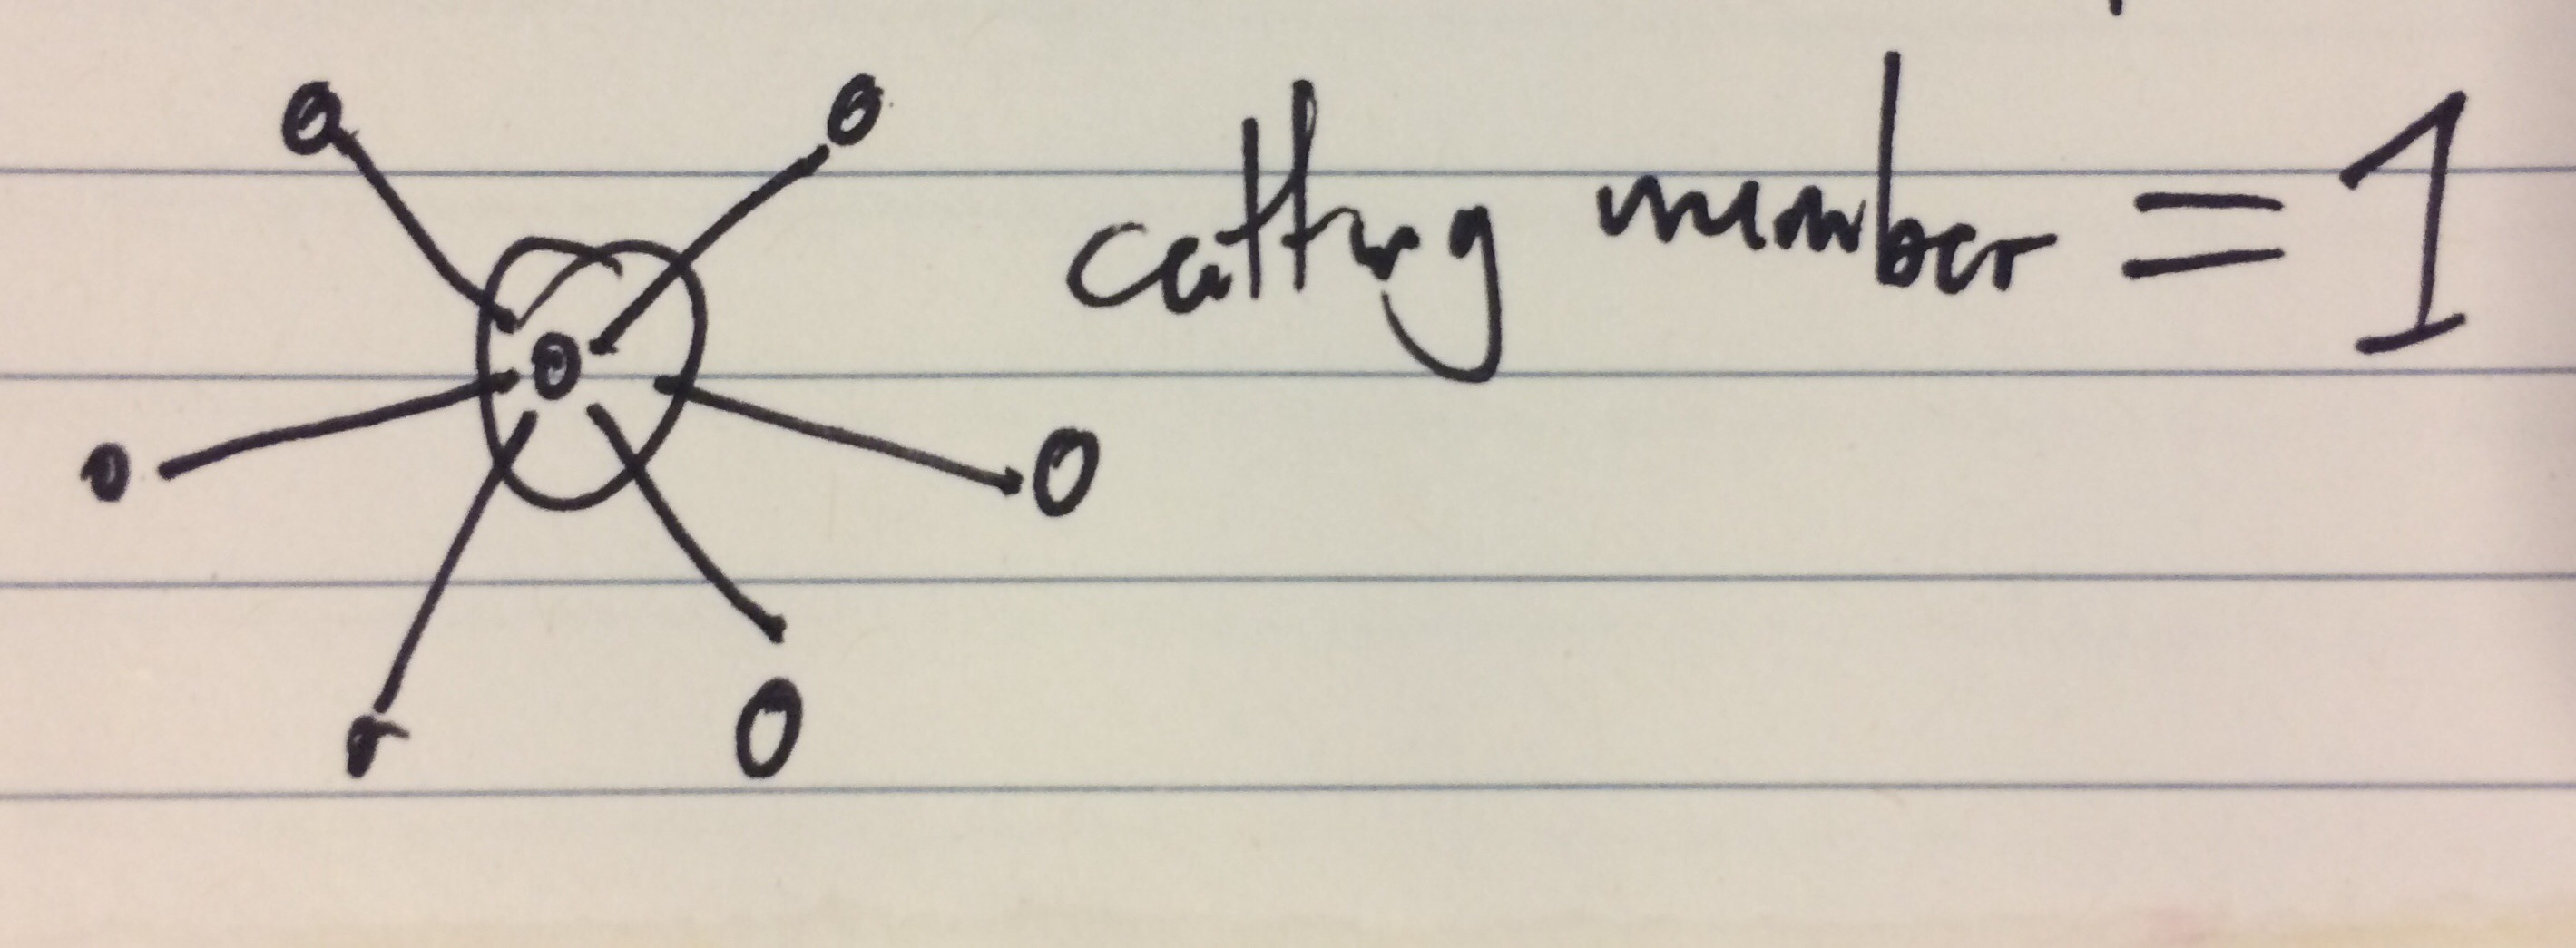
\includegraphics[scale=0.125]{lec2-3}

\subsubsection{Uber (Pathfinding)}

Pathfinding is a graph problem where $V$ represents all the intersections of a map and $E$ is all the roads. For a path $v_1, ... ,v_n$, the length is the number $m$, which is the sum of all the edge weights $\geq 0$, and for 2 connected vertices, we are trying to find the path of the least length. Dijsktra's Algorithm solves this problem.

\subsection{Morphism}

A morphism of graphs $G \mapsto G'$ consists of 2 functions:
\begin{itemize}
	\item{$\gamma_1 : V(G) \mapsto V(G')$}
	\item{$\gamma_2 : E(G) \mapsto E(G')$}
\end{itemize}

$\forall e$, if $e \in E(G)$ has endpoints $v_1, v_2$, this implies that $\gamma_2 (e)$ has endpoints $\gamma_1 (v_1), \gamma_1 (v_2)$.\\
\\
\begin{tcolorbox}
	Note: This definition is more general than the book.
\end{tcolorbox}

An isomorphism is a morphism such that $\gamma_1, \gamma_2$ are both bijective.
\\
\\
\underline{Example of a morphism:} (Note that $\simeq$ denotes a morphism)\\
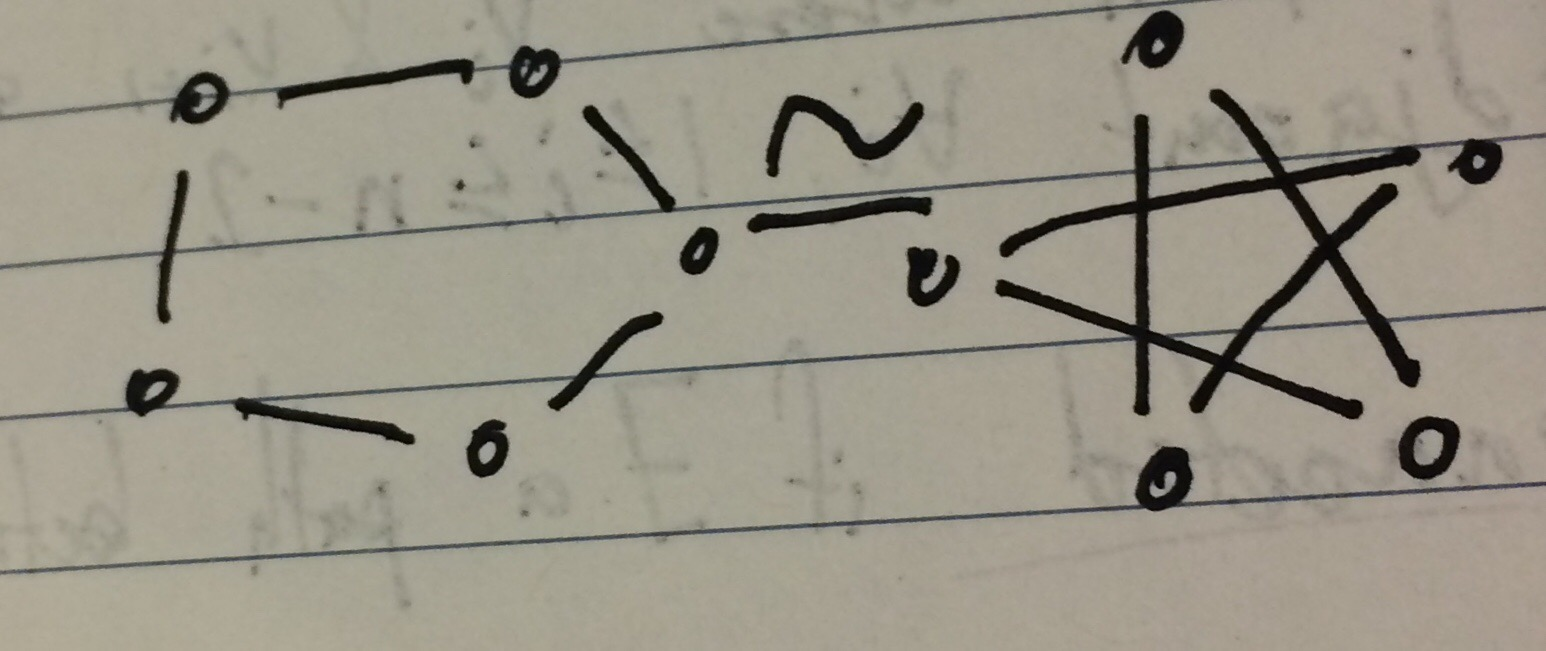
\includegraphics[scale=0.125]{lec2-4}

\newpage

\section{Tuesday, September 12, 2017}

\subsection{More Morphism}

\begin{tcolorbox}[title=Observation 1]
	if $G'$ is simple, there exists a morphism $G \mapsto G'$ and so $\gamma_1 : V(G) \mapsto V(G')$ such that if $e\in E(G)$ has endpoints $v_1, v_2$, then $\gamma_1 (v_1), \gamma_1 (v_2)$ are adjacent.
\end{tcolorbox}

A \textbf{subgraph} of $G$ is a subset $V' \subset V$, $E' \subset E$ such that $Id: (V', E') \mapsto G$ is a morphism.\\
\\
An \textbf{isomorphism} is when a morphism $G \mapsto G'$ is bijective (That there is a one to one relationship between $E \mapsto E'$ and $V \mapsto V'$)\\
\\
\underline{Exercise:} if $(\gamma_1, \gamma_2) : G \mapsto G'$ is an isomorphism, then $(\gamma_1^{-1}, \gamma_2^{-1}) : G' \mapsto G$\\
\\
\underline{Recall:} Bijective implies injective and surjective.

\begin{tcolorbox}[title=Definition: Complement of Simple Graphs]
	The complement of a simple graph $G$ is $\overset{\_\_\_}{G} = (\overset{\_\_\_}{V},\overset{\_\_\_}{E})$ where $V(\overset{\_\_\_}{G}) = V(G)$ and $\overset{\_\_\_}{E}$ does not have any edge in $E$, but if $v_1,v_2 \in V$ are not adjacent, then $v_1,v_2$ are adjacent in $\overset{\_\_\_}{G}$ for all $v_1,v_1 \in V$
\end{tcolorbox}

\underline{Example:}\\
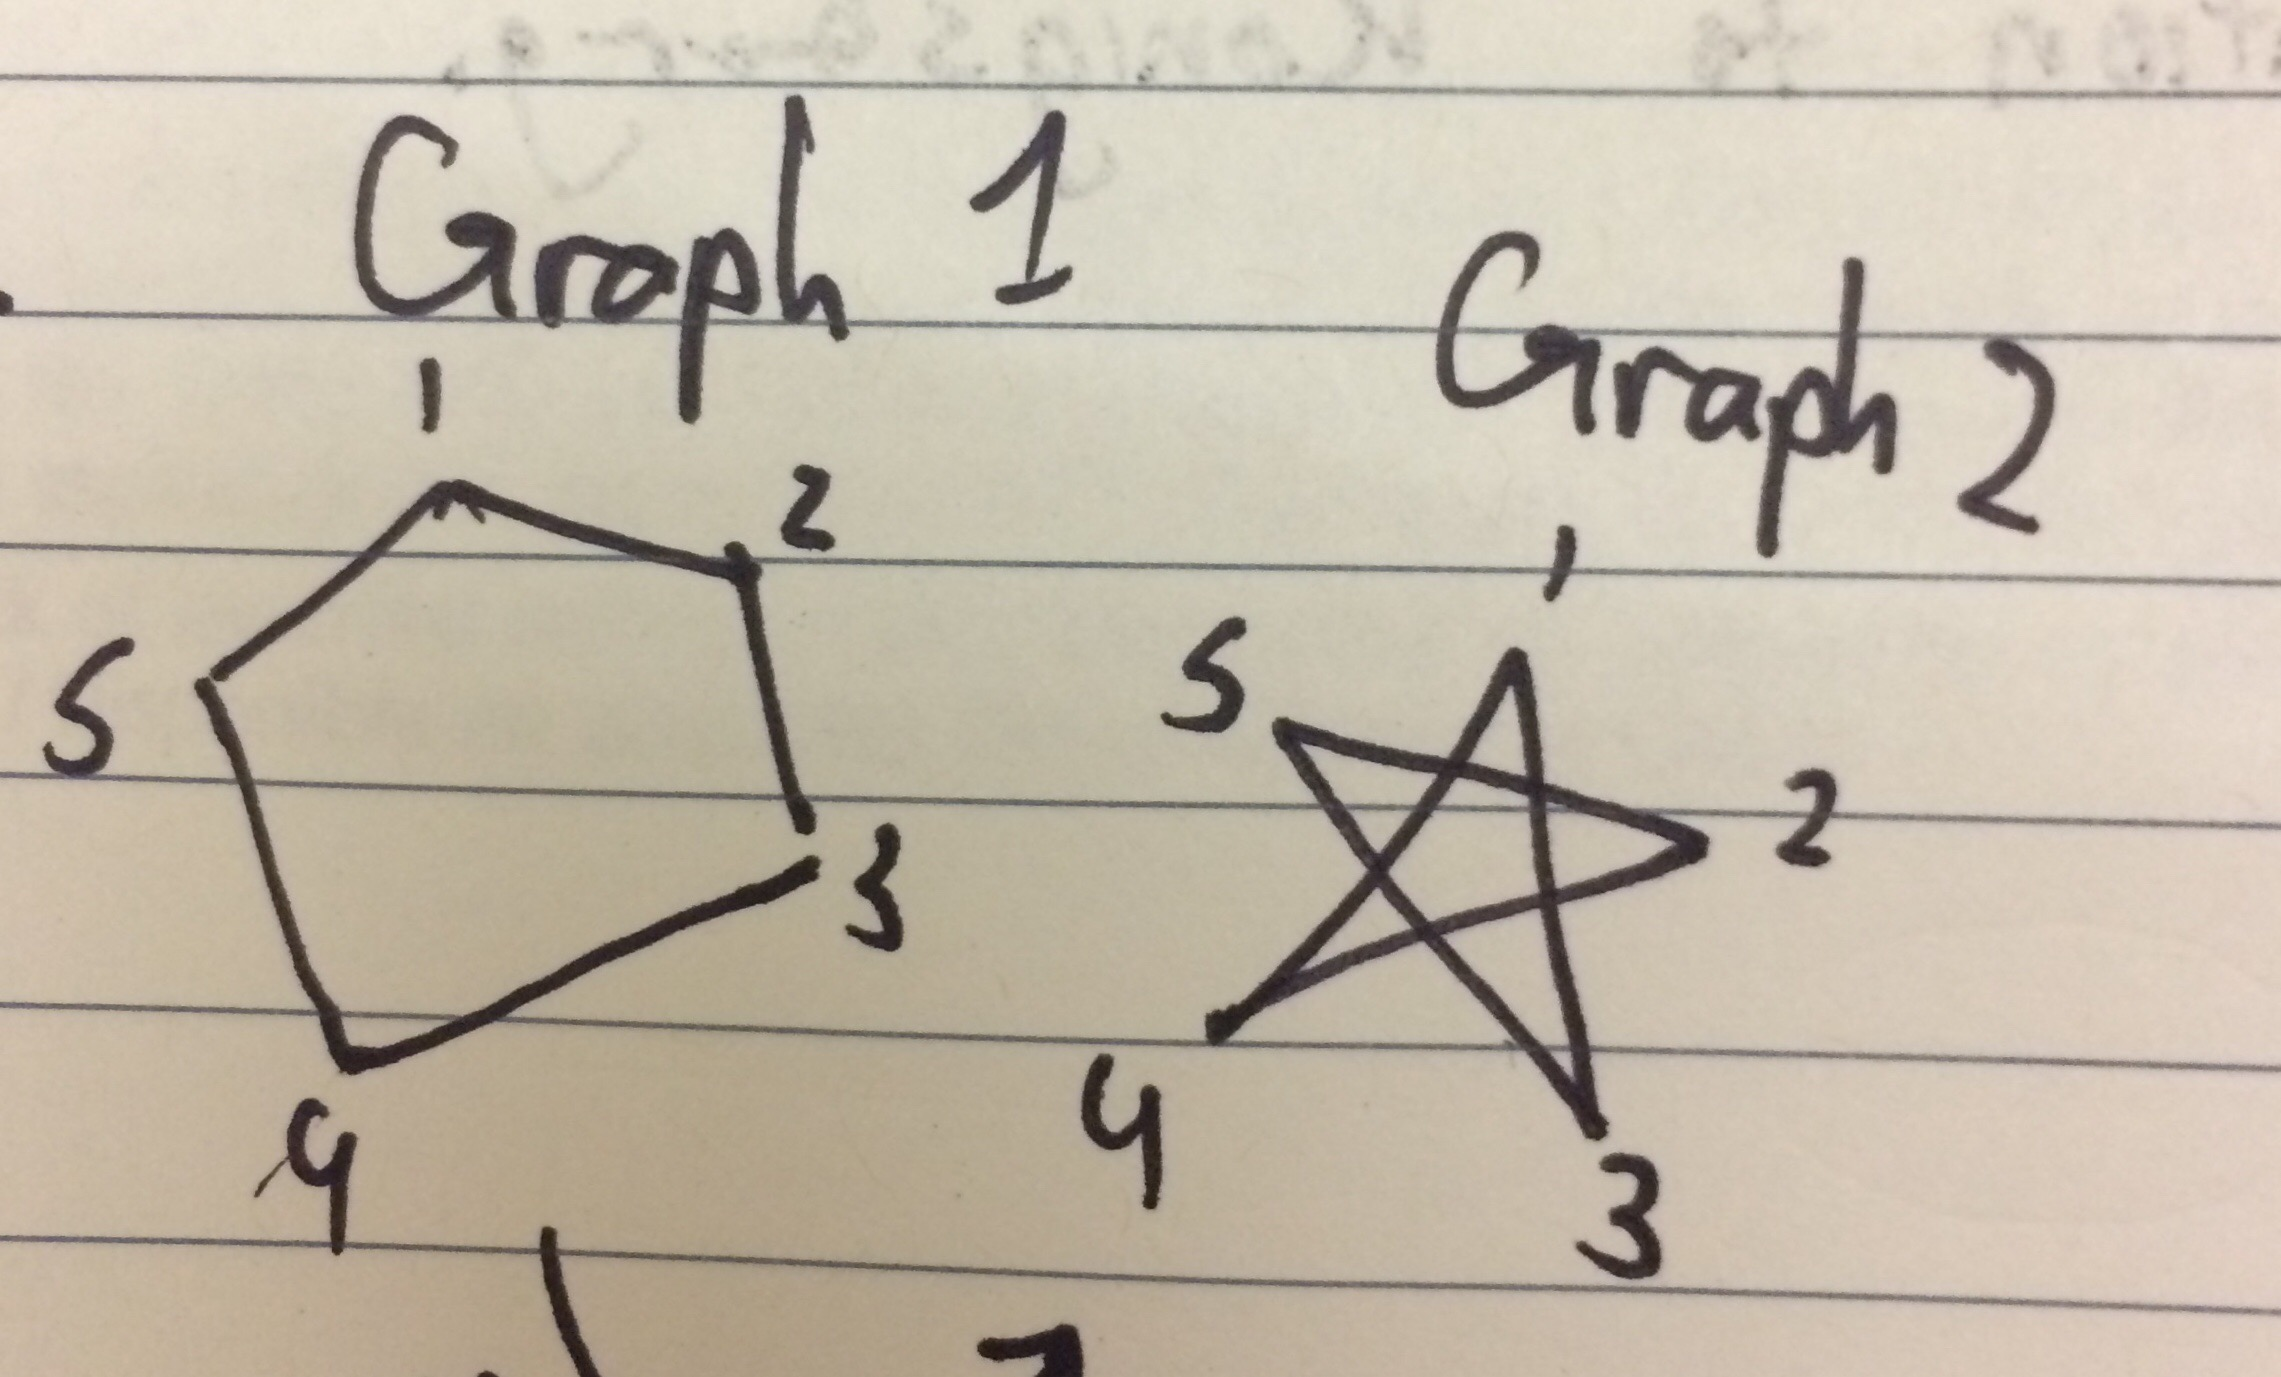
\includegraphics[scale=0.125]{lec3-1}\\
Graph 1 and Graph 2 are complements of each other.

We say a graph is \textbf{self-complementary} if a graph is isomorphic to its complement.

\subsection{Decomposing Graphs}

\begin{tcolorbox}[title=Definition: Union of Graphs]
	if $G_1, G_2$ are two graphs, assume $V(G_1), V(G_2) \subset V$ and $E(G_1), E(G_2) \subset E$. Then for a Graph $G_1 \cup G_2$
	\begin{itemize}
		\item{$V(G_1 \cup G_2) = V(G_1) \cup V(G_2)$}
		\item{$E(G_1 \cup G_2) = E(G_1) \cup E(G_2)$}
	\end{itemize}
\end{tcolorbox}

\underline{Example:}\\
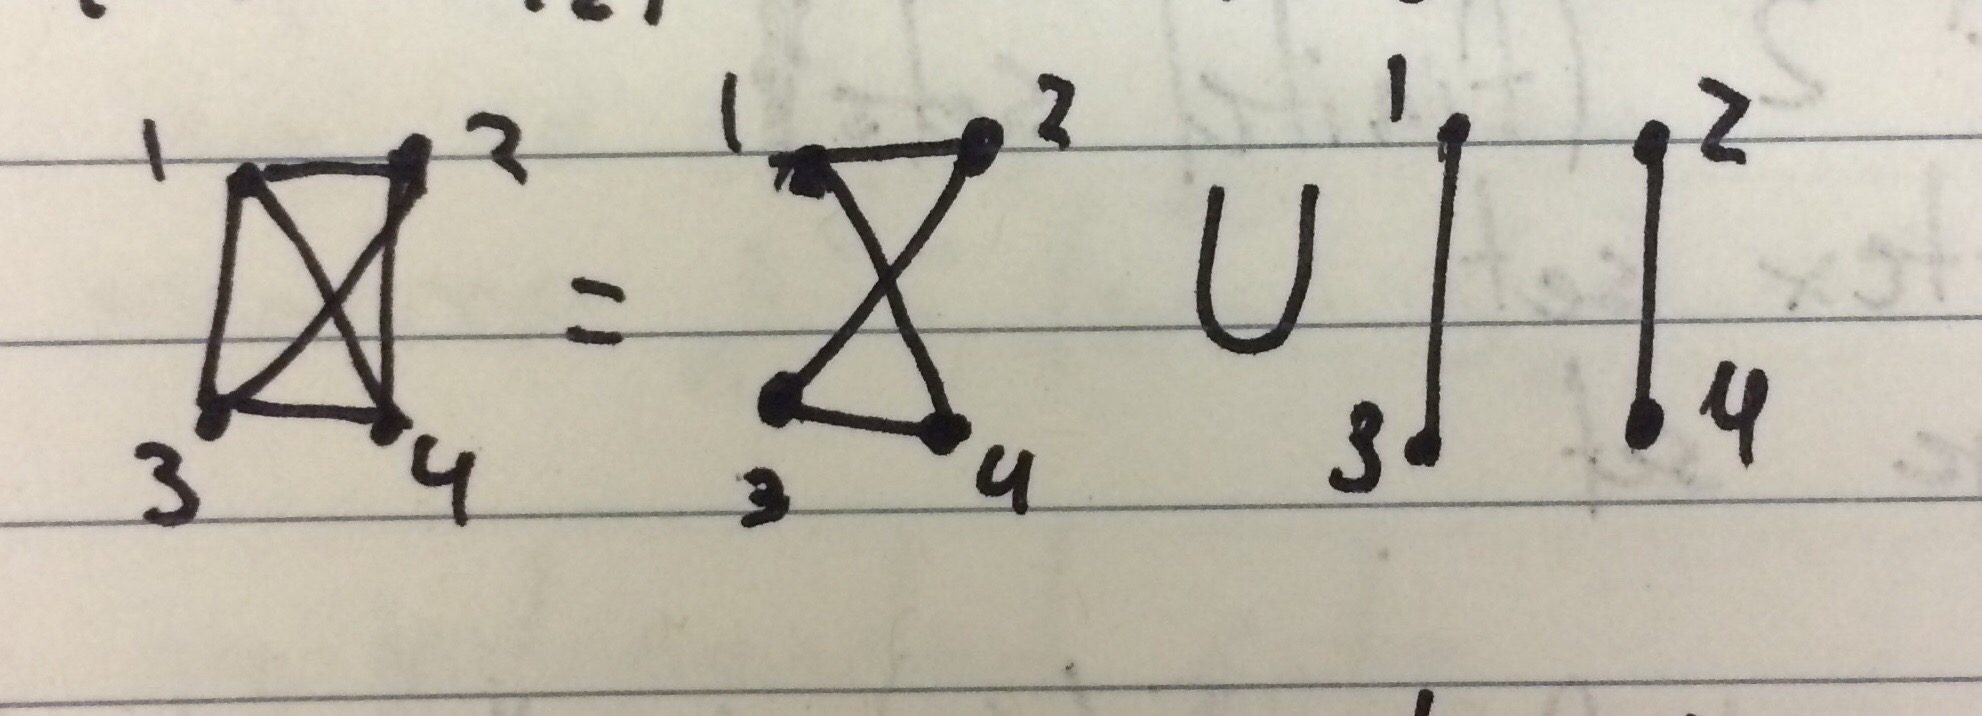
\includegraphics[scale=0.2]{lec3-2}\\

We say $G$ \textbf{decomposes} into $G_1$ and $G_2$ if the following:
\begin{itemize}
	\item{$G_1 \cup G_2 = G$}
	\item{if $\forall e \in E(G)$ there exists one $i$ such that $e\in E(G_i)$ (so if the edges between $G_1$ and $G_2$ don't overlap)}
\end{itemize}

\underline{Example:}\\
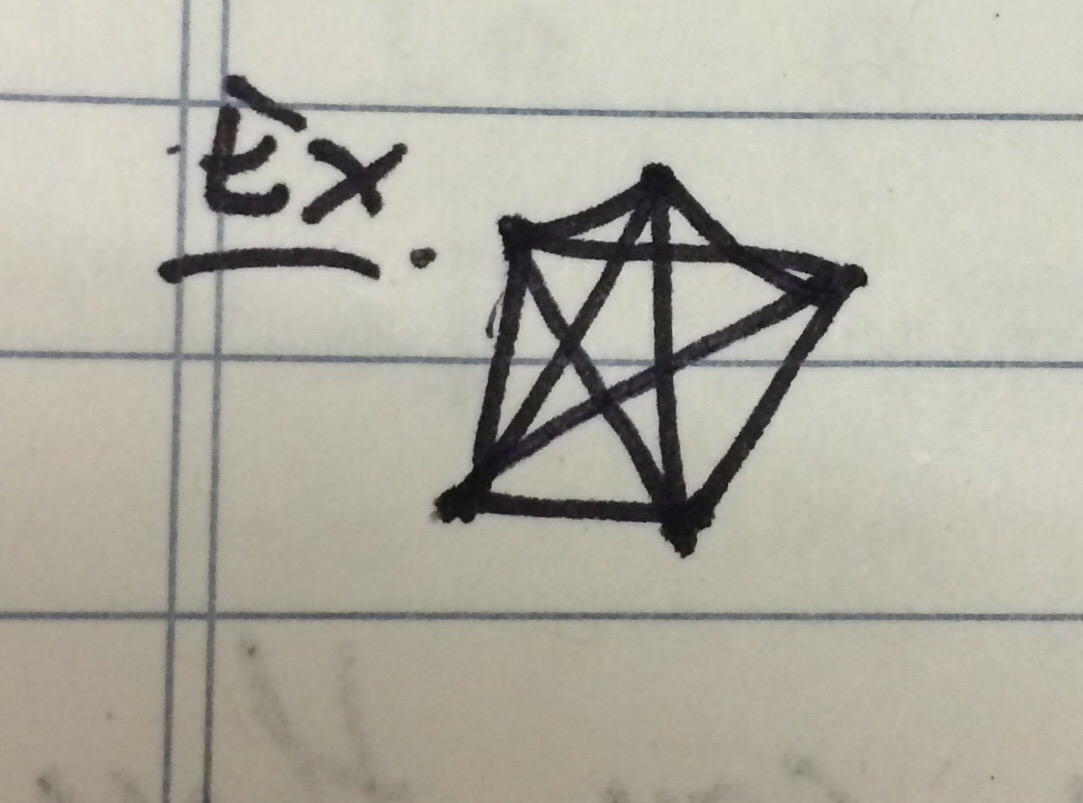
\includegraphics[scale=0.3]{lec3-3}\\
This is $k_5$, the complete simple graph of 5 vertices (complete meaning all vertices are adjacent)\\
\\
\underline{Example:}\\
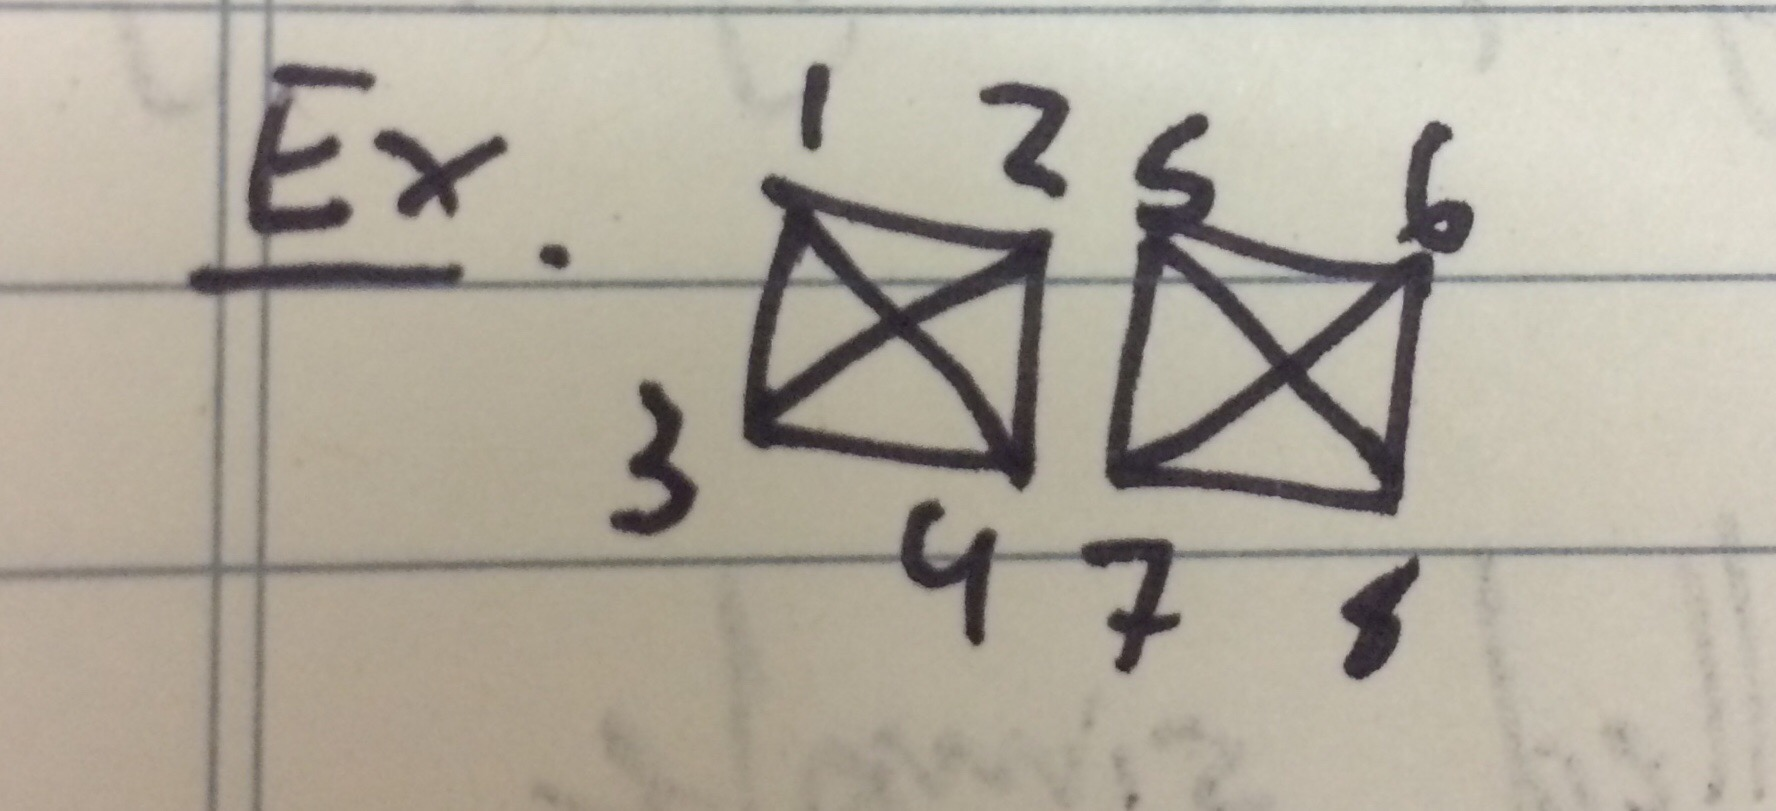
\includegraphics[scale=0.22]{lec3-4}\\
This is the disjoint union of 2 graphs. $G_1 \sqcup G_2$ is the union of 2 graphs with $V(G_1) \cap V(G_2) = \emptyset$

\subsubsection{Connectivity of $G$}

\paragraph{Path} A path is a simple subgraph such that we can order vertices $v_1, ... ,v_{n-1}$ in such a way that exactly $v_i, v_{i+1}$ are adjacent $\forall i$

\paragraph{Cycle} A cycle is a subgraph that is simple and that we the vertices $v_1, ... ,v_{n}$, $v_1 = v_n$ such that exactly $v_i, v_{i+1}$ are adjacent $\forall i$ and that all edges are unique.\\
\\

\underline{Note:} the arrangement of vertices in a path is called a \textbf{walk}, the arrangement of vertices in a cycle is called a \textbf{trail}.\\
\\
we refer to an edge by $(u,v)$ where $u,v$ are the start and end vertices.

\newpage

\section{Friday, September 15, 2017}

\subsection{Equivalence Relations on a set}

\underline{i.e.} Let $X$ be the set of people in a room and the pair $(p_1, p_2) \in R$ if $p_1 \in X$ and $p_2 \in X$ are the same age.\\
\\
An equivalence relation can be thought of as a certain property that is equal between 2+ elements.\\
\\
\begin{tcolorbox}
	\underline{Note:} For $R$ which is the set of people in $X$ that have the same age, you can subdivide $X$ into disjoint subsets of $R$. We can rename $R$ as $x_i$ where $i$ is the age of the people in the set (a partitioned $x$)
	$$\bigcup x_i = X$$
	$$x_i \cap x_j = \emptyset, i \neq j$$
\end{tcolorbox}

\begin{tcolorbox}[title=Definition: Equivalence Relation]
	A set of pairs $R$ is an equivalence relation if it has the following properties:
	\begin{itemize}
		\item{\textbf{Reflexive} : $\forall x \in X, (x,x) \in R$}
		\item{\textbf{Symmetric} : $\forall x,y \in X, (y,x) \in R$ implies $(y,x) \in R$}
		\item{\textbf{Transitive} : $\forall x,y,z \in X, (x,y),(y,z) \in R$ implies $(x,z) \in R$}
	\end{itemize}

\end{tcolorbox}

Some examples include people who like the same colour, have the same age, have the same major,....\\
\\
\underline{Claim:} If $R$ is an equivalence relation, then $X = \{ y : (x,y) \in R \}$ forms a partition.

\begin{proof}
	For notation, we will write $x \sim y$\\
	We need to prove 2 things.\\
	\begin{enumerate}
		\item{$\bigcup_{x\in X} \overset{\_\_\_}{x} = X$}, so we pick $x \in X$ and since $x \sim x$ then that implies that $x \in \overset{\_\_\_}{x}$
		\item{
			Union is disjoint. So we must prove that
			$$(a) \overset{\_\_\_}{x} \cap \overset{\_\_\_}{y} = \emptyset \text{ if } \overset{\_\_\_}{x} \neq \overset{\_\_\_}{y} \text{ iff } (b) \exists z : z\in \overset{\_\_\_}{x} \cup \overset{\_\_\_}{y} \rightarrow \overset{\_\_\_}{x} = \overset{\_\_\_}{y}$$
			
			If we assume $(b)$ is true then:
			\begin{align*}
				&\rightarrow x\sim z, y\sim z\\
				&\rightarrow x\sim z, z\sim y \text{ by symmetry}\\
				&\rightarrow x\sim y \text{ by transitivity}\\
				&\rightarrow y \in x
			\end{align*}
			next we assume $a\in\overset{\_\_\_}{x} \rightarrow x\sim a$, but $y\sim x \rightarrow y\sim a \rightarrow a \in y$
			Therefore we have that $\overset{\_\_\_}{x} \subset \overset{\_\_\_}{y}$ and $\overset{\_\_\_}{y} \subset \overset{\_\_\_}{x}$
		}
	\end{enumerate}
\end{proof}

\begin{tcolorbox}
	\textit{SideNote:} if we start with a partition of $X$ into subsets $(x)\in l $ then the relation $x\sim
y \leftrightarrow x,y$ lie in the same $X$ is an equivalence relation with partition $(x_i)_{i\in l}$
\end{tcolorbox}

\underline{Example:} Take the set of all graphs, say $G,G'$ and $\exists \text{ an isomorphism } G \mapsto G' $ and $G' \mapsto G''$ then $\exists \text{ an ismorphism }  g \circ f : G \mapsto G''$

\begin{tcolorbox}
	\textbf{Reminder:} graph $G$ with vertices $u,v$\\
	$(u,v) = $ path in a simple graph where we can order vertices $u,...,v$ such that only adjacent edges have consecutive endpoints (ordering is a walk)
\end{tcolorbox}

For any graph $G$, say $x,y \in V(G)$

$$x\sim y \leftrightarrow \begin{cases}
	y=x\\
	y \text{ is connected to } x
\end{cases}
$$
is an equivalence relation.\\
\\
For a vertex $v$, the set $\overset{\_\_\_}{v} = \{ y : y \text{ connected is the connected component of } x \text{ to } v \} $\\
\\
\begin{tcolorbox}
	\underline{Note:} The subgraph $\overset{\_\_\_}{x}$ is connected
\end{tcolorbox}

If $u_1, u_2 \in \overset{\_\_\_}{v}$ which imples that $u_1 \sim v, u_2 \sim v$ which implies that $u_1 \sim v, v \sim u_2$ which implies that $u_1 \sim u_2$

\begin{tcolorbox}
	\underline{Result:} Every graph is the disjoint union of common subgraphs, this result characterizes edge cuts and characterizes bipartite graphs
\end{tcolorbox}

\begin{tcolorbox}[title=Definition: Edge Cuts]
	In a graph $G$, an edge creates a cut if the number of connected components of $G \setminus \{ e \}$ increases
\end{tcolorbox}

If an edge lies in a cycle, it is not a cut edge or, a cut edge does not lie in a cycle.\\
\\
\begin{tcolorbox}[title=Thereom]
	An edge is a cut edge iff that edge does not lie on the cycle.
\end{tcolorbox}

\begin{proof}
	Take an edge $e$, we need to show that $G\setminus \{ e \}$ remains connected (which implies that e lies in a cycle).\\
	Assume $G \setminus \{ e \}$ is connected, let $x,y$ be the endpoints of $e$, since $G \setminus \{ e \}$ is connected, there is a path between $x,y \in G \setminus \{ e \}$.\\
	Now assume $e$ lies in a cycle in $G$, we need to show that $G \setminus \{ e \}$, or that there exists a path between nodes $u,v$ where $u$ is an adjacent node to $x$ but is not equal to $y$ and $v$ is an adjacent node to $y$ but is not equal to $x$.\\
	\\
	Now since $G \setminus \{ e \}$ is connected, there is a path between nodes $u$ and $v$ that does not go through edge $e$ and a path that goes through edge $e$ (namely, the path $u,x,y,v$). Therefore $e$ is not an edge cut iff it lies on a cycle. This implies that the negation of this is true, that an edge is an edge cut iff it doesn't lie on a cycle.
\end{proof}

\newpage

\section{Tuesday, September 19, 2017}

\subsection{Konig's Theorem (continued)}

\begin{tcolorbox}
	\underline{Recall:} Can we see when a given graph is bipartite? (A graph $G$ is bipartite if $V(G) = X \sqcup Y$ and $X,Y$ are independent sets)
\end{tcolorbox}

Konig's Theorem states that $G$ is bipartite iff there are no off length cycles.\\
\\
\textbf{Lemma:} In a graph $G$, any odd length walk that is also closed contains a cycle.\\
\\
From this we observe that we can assume that $G$ is connected.\\
\\
\underline{TONCAS (The Obvious Necessary Conditions Are Also Sufficient):} A bipartite graph cannot have odd length cycles.\\
\\
Observe that a cycle must travel through an even number of edges to return to the original vertex.\\
\\
\textit{Now consider the converse of this statement:} If the cycle travels odd edges, the cycle will be on the other side of the partition (so if $V(G) = X \sqcup Y$ and the cycle started at $X$, travelling odd edges will mean the cycle will finish in partition $Y$.)\\
\\
Let $v \in V(G)$\\
$X = \{ u \in V(G) : \text{ the path of minimal length between $v,u$ is even for all $v\in V(G)$ } \}$\\
$Y = \{ u \in V(G) : \text{ the path of minimal length between $v,u$ is odd for all $v\in V(G)$ } \}$
\\
\\
So we know from this that.
\begin{enumerate}
	\item{$G = X \sqcup Y $}
	\item{$X,Y$ are independent}
\end{enumerate}

Assume $X$ is not independent, so let $c$ be an edge between $u, u' \in X$, so take a path $$p: v \rightarrow u \text{ of minimal even length}$$ and a path $$p': u' \rightarrow v \text{ of minimal even length}$$
now consider the path $$v\overset{p}{\rightarrow} u \overset{c}{\rightarrow} u' \overset{p'}{\rightarrow} v$$
This is a closed walk of odd length, therefore there exists a closed cycle of odd length.\\
Therefore there exists a closed walk of odd length iff $X,Y$ are not independent (i.e. a Bipartite graph).

\subsection{Networks}

From this we will look at the Max Flow and Min Cut problem. This involves looking at directed graphs where all the edges in the graph are assigned a flow, which can represent the carrying capacity of trains along a route. This may be important as we may need to know what would be the best way to disrupt the network.

\begin{tcolorbox}[title=Definition: Directed Graph]
	A graph $G$ consists a set of vertices ($V(G)$) and a set of edges ($E(G)$) and
	$$E(G) \mapsto V(G) \times V(G) : e \mapsto (h(e), t(e))$$ where $h(e), t(e)$ refer to the head and tail of edge $e$ respectively.
\end{tcolorbox}

\begin{tcolorbox}[title=Definition: Network]
	A type of directed graph with a source node $s$ that no edge goes into and a sink node $t$ that no edge goes out of. There is also a capacity function $$c : E(G) \mapsto \mathbb{R} \geq 0$$ that assigns a capacity of flow for each edge in $E(G)$
\end{tcolorbox}

\begin{tcolorbox}
	\underline{Remark:} For this week, assume $G$ is simple directed graph, i.e. between any choice of $v_1,v_2 \in V(G)$, there exists at most 1 edge with a head of $v_1$ and a tail of $v_2$. We will also introduce some notation that if there exists an edge from $v_1$ to $v_2$ we denote it as $$v_1 \rightarrow v_2$$
\end{tcolorbox}

\begin{tcolorbox}[title=Definition: Capacity function]
	a capacity function $c: V \times V \mapsto \mathbb{R}\geq 0$ (takes in 2 vertices and returns a positive real number) and is defined by:
	$$c(v_1, v_2) = \begin{cases}
		c(v_1 \rightarrow v_2) &\text{ if }  (v_1 \rightarrow v_2)\in E\\
		0 &\text{ if }  (v_1 \rightarrow v_2)\not\in E\\
	\end{cases}
$$
\end{tcolorbox}
\begin{tcolorbox}[title=Definition: Flow $f$]
	a flow function is defined as $f: E(G) \mapsto \mathbb{R} \geq 0$ with the following properties:
	\begin{itemize}
		\item{$\forall e, f(e) \leq c(e)$}
		\item{for all vertexes v, $f^-(v) = \sum_{u \in V} f(u \rightarrow v)$}
		\item{for all vertexes v, $f^+(v) = \sum_{u \in V} f(v \rightarrow u)$}
		\item{$f^+(v) = f^-(v)$ for all vertices $v$ except for the sink and source nodes $s,t$}
	\end{itemize}
We also define $|f| = f^+(s)=f^-(t)$ as the value of the flow $f$
\end{tcolorbox}

\newpage

\section{Tuesday, September 26, 2017}

\subsection{Flow on a network}

So for some reason, Louis also denotes the value of the flow $f$ as $\partial f$.\\
\\
There are 2 main questions about network flows, and right now we will discuss the one in the form of the min-cut max-flow theorem.\\
\\
Starting from any flow, if it is not the maximal flow, we can construct one, but we must define a few terms first

\begin{tcolorbox}[title=Definition: Cut in a Network]
	Let $G$ be a network, a cut $(S,T)$ is a partition $V(G) = S \sqcup T$, where $s\in S, t \in T$. The \textit{capacity of the cut} is defined as
	$$\sum_{u\in S, v\in T} c(u,v) = c(S,T)$$
\end{tcolorbox}

\begin{tcolorbox}[title=Definition: Minimal Cut]
	Let $G$ be a network, a cut $(S,T)$ is a \textit{minimal cut} if $\forall (S', T')$ cuts of $G$, $$c(S,T) \leq c(S',T')$$
\end{tcolorbox}

\begin{tcolorbox}
	\underline{Recall:} for any flow $f$ and any cut $(S,T)$ on a graph $G$, $\partial f \leq c(S,T)$.\\
	We can also increase any flow until we get a maximum one from the Ford-Fulkerson algorithm.\\
	And for a maximum flow $f'$ and a minimal cut $(S',T')$, we get that $$\partial f' = c(S',T')$$
	Which is the min-cut, max-flow equation
\end{tcolorbox}

The Idea of the Ford Fulkerson Algorithm is that we use the appropriate paths from $s\rightarrow t$ to increase the flow of the network to the maximum flow accordingly.\\
\\
For a network $G$, a capacity function $c$ and a flow $f$.
\begin{itemize}
	\item{for any edge $(u,v)$ where $u,v \in V(G)$, the residual capacity of this edge is defined as $$c_f (u,v) = c(u,v) - f(u,v)$$}
	\item{An augmented path is an (undirected) path in the underlying graph $G$.}
	\item{For any edge, the residual capacity of that edge is strictly positive.}
\end{itemize}

Intuition for the Ford Fulkerson Algorithm:
\begin{enumerate}
	\item{if a flow has an augmented path, the flow cannot be maximal if the path goes from $s$ to $t$.}
	\item{If an augmented path $p$ between $s$ and $t$ exists, then we can adapt $p$ such that $\partial f$ increases and $p$ is no longer augmented.}
	\item{If there exists no augmented path $p$, this means that the path is maximal}
	\item{We use this construction to argue that there exists an obvious min-cut equal to the resulting value of the flow.}
\end{enumerate}

\underline{Example}, consider any path $p: s \rightarrow t$ on graph $G$, let $u,v$ be any 2 nodes in this path where $(u,v)$ is on the path.\\

let $m = \{ c_f (u,v) : (u,v) \in p \} = \{ c(u,v) - f(u,v) : (u,v) \in p \} > 0$ at each edge of the path $p$, replace $f(u,v)$ by $f(u,v) + m$\\
\\
Note that $\partial f$ has increased and that $p$ is no longer augmented.\\
\\
As if $m = c_f (u,v)$, the new flow has the weight of $$f(u,v) + m = f(u,v) + c(u,v) - f(u,v) = c(u,v)$$
\begin{tcolorbox}
	\underline{note:} Adding $m$ to all edges in p yields an increased flow.
\end{tcolorbox}


\end{document}


























